\documentclass[letterpaper,12pt]{article}
\usepackage{amsmath,amsfonts,amsthm,amssymb,graphicx,mathtools,tikz,hyperref}
\usepackage{esvect,esint, subcaption, mathrsfs,comment, quiver, faktor}
\usepackage[onehalfspacing]{setspace}
\usepackage[ddmmyyyy]{datetime}
\renewcommand{\dateseparator}{.}


% place figures and tables where it seems like they should be
\usepackage{float}
\floatplacement{figure}{H}
\floatplacement{table}{H}

% automatically center figures/tables
\makeatletter
\g@addto@macro\@floatboxreset{\centering}
\makeatother

\usepackage{tocvsec2}
\usepackage[bookmarksdepth=subsection]{hyperref}
\usepackage{bookmark}
\usepackage[margin=1in]{geometry}
\usepackage{authblk}
\usepackage{titling}
\setlength{\droptitle}{-1in}

\newcommand{\A}{\mathbb{A}}
\newcommand{\B}{\mathbb{B}}
\newcommand{\C}{\mathbb{C}}
\newcommand{\D}{\mathbb{D}}
\newcommand{\E}{\mathbb{E}}
\newcommand{\F}{\mathbb{F}}
\newcommand{\G}{\mathbb{G}}
\newcommand{\Hb}{\mathbb{H}} %
\newcommand{\I}{\mathbb{I}}
\newcommand{\J}{\mathbb{J}}
\newcommand{\K}{\mathbb{K}}
\newcommand{\Lb}{\mathbb{L}} %
\newcommand{\M}{\mathbb{M}}
\newcommand{\N}{\mathbb{N}}
\newcommand{\Ob}{\mathbb{O}} %
\newcommand{\Pb}{\mathbb{P}} % 
\newcommand{\Q}{\mathbb{Q}}
\newcommand{\R}{\mathbb{R}}
\newcommand{\Sb}{\mathbb{S}} % 
\newcommand{\T}{\mathbb{T}}
\newcommand{\U}{\mathbb{U}}
\newcommand{\V}{\mathbb{V}}
\newcommand{\W}{\mathbb{W}}
\newcommand{\X}{\mathbb{X}}
\newcommand{\Y}{\mathbb{Y}}
\newcommand{\Z}{\mathbb{Z}}
\newcommand{\Ac}{\mathcal{A}}
\newcommand{\Bc}{\mathcal{B}}
\newcommand{\Cc}{\mathcal{C}}
\newcommand{\Dc}{\mathcal{D}}
\newcommand{\Ec}{\mathcal{E}}
\newcommand{\Fc}{\mathcal{F}}
\newcommand{\Gc}{\mathcal{G}}
\newcommand{\Hc}{\mathcal{H}} %
\newcommand{\Ic}{\mathcal{I}}
\newcommand{\Jc}{\mathcal{J}}
\newcommand{\Kc}{\mathcal{K}}
\newcommand{\Lc}{\mathcal{L}} %
\newcommand{\Mc}{\mathcal{M}}
\newcommand{\Nc}{\mathcal{N}}
\newcommand{\Oc}{\mathcal{O}} %
\newcommand{\Pc}{\mathcal{P}} % 
\newcommand{\Qc}{\mathcal{Q}}
\newcommand{\Rc}{\mathcal{R}}
\newcommand{\Sc}{\mathcal{S}} % 
\newcommand{\Tc}{\mathcal{T}}
\newcommand{\Uc}{\mathcal{U}}
\newcommand{\Vc}{\mathcal{V}}
\newcommand{\Wc}{\mathcal{W}}
\newcommand{\Xc}{\mathcal{X}}
\newcommand{\Yc}{\mathcal{Y}}
\newcommand{\Zc}{\mathcal{Z}}

\renewcommand\qedsymbol{$\blacksquare$}
\renewcommand{\bar}[1]{\overline{#1}}
\renewcommand{\epsilon}{\varepsilon}

\newcommand{\ita}[1]{\textit{#1}}
\newcommand{\com}[2]{#1\backslash#2}
\newcommand{\oneton}{\{1,2,3,...,n\}}
\newcommand\idea[1]{\begin{gather*}#1\end{gather*}}
\newcommand\ef{\ita{f} }
\newcommand\eff{\ita{f}}
\newcommand\proofs[1]{\begin{proof}#1\end{proof}}
\newcommand\inv[1]{#1^{-1}}
\newcommand\setb[1]{\{#1\}}
\newcommand\en{\ita{n }}
\newcommand{\vbrack}[1]{\langle #1 \rangle}
\DeclareMathOperator{\rank}{rank}
\DeclareMathOperator{\ord}{ord}
\DeclareMathOperator{\Aut}{Aut}
\DeclareMathOperator{\Span}{span}
\DeclareMathOperator{\Int}{Int}
\DeclareMathOperator{\cl}{cl}
\DeclareMathOperator{\diam}{diam}
\DeclareMathOperator{\stab}{stab}

\theoremstyle{plain}
\newtheorem{theorem}{Teorema}
\newtheorem{axiom}{Axioma}
\newtheorem{lemma}[theorem]{Lema}
\newtheorem{proposition}[theorem]{Proposici\'on}
\newtheorem{postulate}{Postulado}
\newtheorem*{corollary}{Corolario}

\theoremstyle{definition}
\newtheorem*{definition}{Definici\'on}
\newtheorem{conjecture}{Conjetura}
\newtheorem{example}{Ejemplo}
\newtheorem*{homework}{Tarea}

\theoremstyle{remark}
\newtheorem*{claim}{Reclamo}
\newtheorem*{note}{Nota}

\pretitle{
    \begin{center}
        \fontsize{14pt}{1em}
        \bfseries\selectfont
            MATE6201-0U1 \\
            Prof. Luis A. Medina \\
            10.00 - 11.20 \\
            CNL-A-207 \\
            \vspace{14pt}
}

\posttitle{\end{center}}
\preauthor{\begin{center}\fontsize{12pt}{1em}\selectfont}
\postauthor{\end{center}}
\predate{\begin{center}\fontsize{12pt}{1em}\selectfont}
\postdate{\end{center}}

% section heading formatting
\renewcommand{\thesection}{\Roman{section}.}

\usepackage{sectsty}
\sectionfont{\centering\fontsize{12pt}{1em}\selectfont}

\title{Algebra Moderna}

%%%%%%%%%%%%%%%%%%%%%%%%%%%%%%%%%%%%%%%%%%%%%%%%%%%%%%%%%%%%%%%%%%%%%%%%%%%%%%%%
% Your names go here (one should be underlined)
%%%%%%%%%%%%%%%%%%%%%%%%%%%%%%%%%%%%%%%%%%%%%%%%%%%%%%%%%%%%%%%%%%%%%%%%%%%%%%%%
\author{Alec Zabel-Mena}
\affil{Universidad de Puerto Rico, Recinto de Rio Piedras}

\begin{document}
\maketitle
\section*{Lectura 1: Grupos y Subgrupos}

\begin{definition}
    Sea $G$ un conjunto no vacio junto a una operaci\'on binaria  $\cdot$.
    Decimos que el par  $(G,\cdot)$ es un \textbf{grupo} si:
    \begin{enumerate}
        \item[(1)] $a \cdot b \in G$ para $a,b \in G$.

        \item[(2)] $a \cdot (b \cdot c)= (a \cdot b) \cdot c$, para $a,b,c \in G$

        \item[(3)] Existe un $e \in G$ tal que  $a \cdot e=e \cdot a=a$ para
            toda  $a \in G$.

        \item [(4)] Para toda $a \in G$, existe una  $\inv{a} \in G$ tal que $a
            \cdot \inv{a}=\inv{a} \cdot a=e$.
    \end{enumerate}
    Si $a \cdot b = b \cdot a$ para toda  $a,b \in G$, entoces decimos que  $G$
    es un grupo  \textbf{Abeliano}.
\end{definition}

\begin{example}\label{}
    \begin{enumerate}
        \item[(1)] Los naturales $\N$ junto a la multiplicaci\'on es  satisface
            los primeros tres axiomas, pero no es un grupo.

        \item[(2)] El grupo mas peque\~no es el conjunto $\{e\}$, que denotamos
            como $\vbrack{e}$. $\vbrack{e}$ es un grupo Abeliano.

        \item[(3)] Los enteros $\Z$ junto con adici\'on  $+$ forma un grupo
            Abeliano.

        \item[(4)] El conjunto $GL(n,\R)$ de matrices $n \times n$ con entradas
            reales, nosingular forman un grupo con respecto a multiplicaci\'on
            de matrices. $GL(n,\R)$ no es un grupo Abeliano.

        \item[(5)] Sea $S$ cualquier conjunto y  $A(S)$ el conjunto de todas las
            permutaciones de de elementos de $S$. Entonces  $A(S)$ es un grupo
            no Abeliano con respecto a composicion de funci\'ones, $\circ$. Si
            $S$ tiene  $n$ elementos, entonces  $A(S)=S_n$.
    \end{enumerate}
\end{example}

\begin{definition}
    Sea $G$ un grupo. El \textbf{orden} de un grupo es su cardinalidad, y
    escribimos $\ord{G}=|G|$. Decimos que $G$ es  \textbf{finito} si $\ord{G}$
    es finito; de lo contrario, $G$ es  \textbf{infinito}.
\end{definition}

\begin{definition}
    Sea $G$ un grupo, y  $a \in G$. El  \textbf{orden} de $a$, denotado
    $\ord{a}$, es el menor entero positivo $n$ tal que  $a^n=e$ y escribimos
    $\ord{a}-n$. Si tal $n$ no existe, entonces decimos que $a$ es de orden
    \textbf{infinita}, y decimos que $a$ es un elemento  \textbf{torsi\'on}.
\end{definition}

\begin{example}\label{}
    \begin{enumerate}
        \item[(1)] Considera $\C^*=\com{\C}{0}$, entonces $\C^*$ tiene orden
            infinita, note que si $\exp(\frac{2i\pi}{5}) \in \C^*$, entonces
            $\alpha \neq 1$, para $j \neq 1,2,3,4$, pero $\alpha^5=1$. Entonces
             $\ord{\alpha}=5$.

         \item[(2)] Considere $A \in GL(6,\R)$ con la forma
             \begin{equation*}
               A=\begin{pmatrix}
                     0 & 0 & 0 & 0 & 1 & 0 \\
                     0 & 0 & 0 & 0 & 0 & 1 \\
                     1 & 0 & 0 & 0 & 0 & 0 \\
                     0 & 1 & 0 & 0 & 0 & 0 \\
                     0 & 0 & 1 & 0 & 0 & 0 \\
                     0 & 0 & 0 & 1 & 0 & 0 \\
                 \end{pmatrix}
             \end{equation*}
            Entonces
             \begin{equation*}
               A^3=\begin{pmatrix}
                     1 & 0 & 0 & 0 & 0 & 0 \\
                     0 & 1 & 0 & 0 & 0 & 0 \\
                     0 & 0 & 1 & 0 & 0 & 0 \\
                     0 & 0 & 0 & 1 & 0 & 0 \\
                     0 & 0 & 0 & 0 & 1 & 0 \\
                     0 & 0 & 0 & 0 & 0 & 1 \\
                 \end{pmatrix}
             \end{equation*}
             entonces, $A^3=I$.

         \item[(3)] En $\R^*=\com{\R}{0}$, $\R^*$ es infinito, y  $\ord{2}$ es
             infinito.
    \end{enumerate}
\end{example}

\begin{definition}
    Sea $G$ un grupo y  $H \subseteq G$ no vacio. Entonces decimos que  $H$ es
    un  \textbf{subgrupo} de $G$ si  $H$ es un grupo bajo la misma opearaci\'on
    de  $G$. Escribimos  $H \leq G$.
\end{definition}

\begin{example}\label{}
    \begin{enumerate}
        \item[(1)] Considere $GL(n,\R)$ y sea $SL(n,\R)$ los elementos $A \in
           GL(n,\R)$ tales que $\det{A}=1$. Entonces $SL(n,\R) \leq GL(n,\R)$.

       \item[(2)] Sea $C(\R)$ el conjunto de todas las funciones continuas sobre
           $\R$. Entonces  $C(\R)$ es un grupo bajo la suma de funci\'ones $+$.
           Sea $C^1(\R)$ el conjunto primer difirenciable continua de funciones
           sobre $\R$. Observe lo siguiente:
           \begin{enumerate}
               \item[(a)] $(f+g)'=f'+g'$
               \item[(b)] $f'+(g+h)'=(f+g)'+h'$.
               \item[(c)] $c'=0$, entonces $0 \in C^1(\R)$
               \item[(d)] $f'-f'=-f'+f'=0$.
           \end{enumerate}
           Como todos los funciones de arriba tambien son continuas, vemos que
           $C^1(\R) \leq C(\R)$.
    \end{enumerate}
\end{example}

\begin{lemma}\label{}
    Sea $G$ un grupo y  $H \subseteq G$ no vacio. Si tenemos que $ab \in H$,
    implicat que $a\inv{b} \in H$, entonces $H \leq G$.
\end{lemma}
\begin{proof}
    Como $H \neq \emptyset$, sea  $a \in H$. Entonces $a\inv{a}=e \in H$. Luego,
    tambien tenemos qie $e\inv{a}=\inv{a} \in H$. Finalmente, tenemos que si $b
    \in H$, entonces  $a\inv{b} \in H$, por lo tanto $\inv{b} \in H$, entonces
    $a\inv{(\inv{b})}=ab \in H$.
\end{proof}

\begin{example}\label{}
    \begin{enumerate}
        \item[(1)] Considere a los enteros pares $2\Z$. Sean  $2n,2m \in 2\Z$.
            Noten que $2n-2m=2(n-m) \in 2\Z$. Entonces $2\Z \leq \Z$.

        \item[(2)] Si $G$ es un grupo, entonces  $\vbrack{e}$ y $G$ son
            subgrupos de  $G$. Llamamos a $\vbrack{e}$ el grupo
            \textbf{trivial}.

        \item[(3)] Si $G$ es un grupo, y  $a \in G$, entonces el conjunto
            $\vbrack{a}=\{a^j : j \in \Z\}$ es un subgrupo de $G$, llamado el
            \textbf{subgrupo generado por $a$}.

        \item[(4)] Si $G$ es un grupo, y  $a \in G$, entonces  $C(a)=\{g \in G :
            ag=ga\}$ y $Z(G)=\{g \in G : ag=ga \text{ para toda } a \in G\}$ son
            subgrupos. Nota que $Z(G)=\bigcap{C(a)}$. Llamamos a $C(a)$ el
            \textbf{cnetralizador} de $a$ y  $Z(G)$ el \textbf{centro} de $G$.

        \item[(5)] Sea $G$ un grupo y  $H \leq G$, y sea  $a \in G$, entonces
        $\inv{a}Ha \leq G$. Llamamos a $\inv{a}Ha$ el \textbf{conjugado} de $H$
         \textbf{con respecto} a $a$.
    \end{enumerate}
\end{example}

\begin{definition}
    Suponga que $G$ y  $H$ son grupos. Un mapa  $\phi:G \rightarrow H$ se llama
    un \textbf{homomorphismo} si para toda $a,b \in G$,
    $\phi(ab)=\phi(a)\phi(b)$. Si $\phi$ es  $1-1$ y sobre, entonces lo llamamos
    un  \textbf{isomorphismo}. Si $\phi$ es un isomorphismo, y  $G=H$, entonces
    llamamos a  $\phi$ un  \textbf{automorphismo}.
\end{definition}

\section*{Lecture 2: Smallest Infinite Cardinality}

\begin{definition}
    A set $A$ is  \textbf{countably infinite} if there exists a $1-1$ map $f:\N
    \rightarrow A$ of $\N$ onto  $A$.
\end{definition}
\begin{remark}
    That is we can put $A$ into countable order and represent it as an
    increasing sequence $A=\{a_n\}_{n \in \N}$ where each $a_n$ is distinct for
    all  $n$.
\end{remark}

\begin{example}\label{}
    Both $\N$ and  $2\N$ are countable. Consider the identity map  $i:\N
    \rightarrow \N$ and the map $f:\N \rightarrow 2\N$ defined by $n \rightarrow
    2n$.
\end{example}

\begin{theorem}\label{thm_2.1}
    A set $A$ is finite if, and only if there is no  $1-1$ map of $A$ onto a
    subset of itself.
\end{theorem}
\begin{corollary}
    Every infinite set countains a countable subset.
\end{corollary}

\begin{theorem}\label{}
    A countable union of sets is countable.
\end{theorem}
\begin{proof}
    Let $A$ and  $B$ be nonempty countable sets. Then there exists nonrepeating
    increaseing sequences  $A=\{a_n\}$ and $B=\{b_m\}$. Then take $A \cup
    B=\{a_n,b_m\}$, and delete any repeated members. Then we can say that $A
    \cup B=\{c_k\}$ where $c_k=a_k$ for  $k$ odd, and  $c_k=b_k$ for  $k$ even.
    Then  $A \cup B$ is countable.

    Now suppose that  $\{A_n\}$ is a collection of countable sets. Then we have
    the following:
    \begin{align*}
        A_1     &=      a_{11} \ a_{12} \ \dots \ a_{1n} \ \dots \\
        A_2     &=      a_{21} \ a_{22} \ \dots \ a_{2n} \ \dots \\
        A_3     &=      a_{31} \ a_{32} \ \dots \ a_{3n} \ \dots \\
                \vdots                              \\
        A_n     &=      a_{n1} \ a_{n2} \ \dots \ a_{nn} \ \dots \\
                \vdots                                \\
    \end{align*}
    Construct the set:
    \begin{equation*}
        A=\{a_{11},a_{12},a_{21},a_{13},a_{22},a_{31}, \dots\}
    \end{equation*}
    Then $A$ is countable and $A=\bigcup{A_n}$.
\end{proof}

\begin{example}\label{}
    \begin{enumerate}
        \item[(1)] $-\N$ is countable, then  $-\N \cup \N=\Z$ is also countable,
            which makes $\Z$ countable.

        \item[(2)]  Consider the rational numbers $\Q=\{\frac{p}{q} : p,q \in
            \Z\}$. Let $\frac{\Z}{n}=\{\frac{p}{n} : p \in \Z\}$ for some $n \in
            \com{\N}{\{0\}}$. Then notice that  $\frac{\Z}{n}$ is countable and
            that $\Q=\bigcup{\frac{\Z}{n}}$, which makes $\Q$ countable as well.
    \end{enumerate}
\end{example}

\begin{lemma}\label{}
    Let $A$ and  $B$ be two countably finite sets. Then  $A \times B$ is
    countable.
\end{lemma}
\begin{proof}
    Take $A \times B=(\bigcup{A_n}) \times \{b_n\}$, where $b_n \in B$.
\end{proof}

\begin{example}\label{}
    \begin{enumerate}
        \item[(1)] Let $P$ be the set of all polynomials with integer
            coefficients. Let  $P_i$ be the set of all polynomials of degree
            $\deg=i$. Then we have the following:
            \begin{align*}
                P_0     &\simeq     \Z      \\
                P_1     &\simeq     \Z \times \Z        \\
                        \vdots              \\
                P_n     &\simeq     \Z \times \Z \times \dots \times \Z        \\
                        \vdots                      \\
            \end{align*}
            Then we have that $P \simeq \bigcup{P_i}$. Since each $P_i$ is
            countable, so is  $\bigcup{P_i}$, so by isomorphism, $P$ must also
            be countable.

        \item[(2)] Let $\Ac=\{x \in \C : \text{ there exists a polynomial with
                integer coefficients } p \text{ such that } p(x)=0\}$ be the set
                of all algebraic numbers over $\C$. Then we have  $\Q \subseteq
                \Ac$, since the polynomial $z^2+1=0$ has complex roots. $\Ac$
                is countable.
    \end{enumerate}
\end{example}

\begin{theorem}\label{}
    Let $A$ be a set, then  $|A|<|2^A|$.
\end{theorem}
\begin{proof}
    We have that by definition, $|A|>|2^A|$ is impossible, so suppose that
    $|A|=|2^A|$. Then there exists a $1-1$ map  $f:A \rightarrow 2^A$ of $A$
    onto its powerset. Then we have that for each  $a \in A$,  $f(a) \subseteq
    A$. Now, let $A_0=\{x \in A : x \notin f(x)\}$. Since $f$ is onto, there is
    an  $x_0 \in A$ with $f(x_0)=A_0$. Now, if $x \in f(x_0)$, we get that $x
    \in A_0$, which means that $x_0 \notin f(x_0)$. This cannot happen; so it
    must be that $x_0 \notin f(x_0)$, but then we get that $x_0 \in A_0$, which
    forces $x_0 \in f(x_0)$. A contradiction! Therefore it must be that
    $|A|<|2^A|$
\end{proof}

\begin{example}\label{}
    $|\N|<|2^\N|$
\end{example}

Now consider the set of real numbers $\R$. We have the following theorems.

\begin{theorem}\label{}
    $\R$ is a field.
\end{theorem}

\begin{theorem}\label{}
    $\R$ is a totally ordered set.
\end{theorem}
\begin{corollary}
    The following are true for all $a,b,c \in \R$.
    \begin{enumerate}
        \item[(1)] $a>b$ impl ies that $a+c>b+c$.

        \item[(2)] $a>b$ and  $c>0$ implies  $ac>bc$.

        \item[(3)] For all $a>0$ and  $b>0$, there exists an  $n \in \N$ such
            that  $an>b$  (Property of Archimedes).
    \end{enumerate}
\end{corollary}

\begin{theorem}\label{}
    $\R$ has the least upperbound property. That is, if  $\{a_n\}$ is an
    increasing sequence of real numbers bounded above by $b$, then  $\sup{\{a_n\}}
    \in \R$.
\end{theorem}

\section*{Lectura 3: Categor\'ias y Funtores.}

\begin{definition}
    Definimos una \textbf{clase} de ser una colecci\'on de objetos tal que s\'i
    $T$ y  $A$ son clases, entonces  $A \notin T$.
\end{definition}

\begin{definition}
    Una \textbf{categor\'ia} $\Cc$ es un clase de objetos denotados por
    $\obj{\Cc}$ junto a una colecci\'on de conjuntos $\Hom{(X,Y)}$,  para
    cualquieras $X,Y \in \obj{\Cc}$, de \textbf{morfismos} de $X$ hac\'ia $Y$,
    cuyas elementos estan denotados $f:X \rightarrow Y$ \'o $X \xrightarrow{f}
    Y$, y una operac\i\'on binaria $\circ:\Hom{(X,Y)} \times \Hom{(Y,Z)}
    \rightarrow \Hom{(X,Z)}$ llamado \textbf{composici\'on} tal que si $f:X
    \rightarrow Y$ y $g:Y \rightarrow Z$ son morfismos, entonces $g \circ f:X
    \rightarrow Z$ es un morfismo y:
    \begin{enumerate}
        \item[(1)] $\Hom{(X,Y)}$ y $\Hom{(A,B)}$ son disjuntas.

        \item[(2)] La composici\'on $\circ$ es associativa s\'i esta definido.
            Es decir, sy  $g \circ (f \circ h)$ \'o $(g \circ g) \circ h$
            existen en $\Hom{(X,Y)}$, entonces $g \circ (f \circ h)=(g \circ f)
            \circ g$.

        \item[(3)] $\Hom{(X,X)}$ no es vac\'io y existe al menos un morfismo
            $1_X:X \rightarrow X$, llamado la \textbf{identidad} de $X$, tal que
            $1_X \circ f=f$ y  $g \circ 1_X=g$ para morfismos  $f:X \rightarrow
            Y$ y $g:Z \rightarrow X$, para cualquieras objetos $X,Y,Z \in
            \obj{\Cc}$
    \end{enumerate}
\end{definition}

\begin{definition}
    Sea $\Cc$ una categor\'ia. Se llama el conjunto $\Mc_\Cc$  \textbf{los
    morfismos de la categor\'ia} donde $\Mc_\Cc$ es la union de todos los
    conjuntos $\Hom{(X,Y)}$ para todos $X,Y \in \obj{\Cc}$.
\end{definition}

\begin{figure}[h]
    \centering
    \[\begin{tikzcd}
	X &&& Y &&& Z
	\arrow["f", from=1-1, to=1-4]
	\arrow["g", from=1-4, to=1-7]
	\arrow["{g \circ f}"', curve={height=30pt}, from=1-1, to=1-7]
\end{tikzcd}\]
    \caption{Un ejemplo de composici\'on de morfismos de una categor\'ia}
    \label{fig_6}
\end{figure}

\begin{figure}[h]
    \centering
    \[\begin{tikzcd}
	X & X &&& Y & Y
	\arrow[curve={height=12pt}, from=1-2, to=1-5]
	\arrow[curve={height=-12pt}, from=1-2, to=1-5]
	\arrow[from=1-2, to=1-5]
	\arrow["{1_X}", from=1-2, to=1-1]
	\arrow["{1_Y}", from=1-5, to=1-6]
	\arrow[curve={height=24pt}, from=1-5, to=1-2]
	\arrow[curve={height=-24pt}, from=1-5, to=1-2]
\end{tikzcd}\]
    \caption{Morfismos entre dos objetos $X$ y  $Y$ de una categor\'ia
    incluyendo las identidades de $X$ y $Y$}
    \label{fig_7}
\end{figure}

\begin{example}\label{}
    \begin{enumerate}
        \item[(1)] Considere la categor\'ia $\Cc=\Conj$, donde  $\boj{\Cc}$ es
            la clase de todo los conjuntos. Los morfismos de $\Cc$ son
            funci\'ones  $f:X \xrightarrow{} Y$ de un conjunto $X$ hac\'ia un
            conjunto  $Y$.

        \item[(2)] Sea $\Cc=\Top$ la categor\'ia de espacios topol\'ogicos,
            donde  $\obj{\Cc}$ es la colecci\'on de todas las espacios
            topol\'ogicos. Los morfismos de $\Top$ son funci\'ones continuas
            entre espacios topologicos. Es decir, $\Hom{(X,Y)}=\{f : f:X
            \xrightarrow{} Y \text{ es continua}\}$. La composici\'on de
            morfismos es la composicion de funciones usual.

        \item[(3)] Sea $\Cc=\Grp$ la categor\'ia de grupos, cuyas objetos son
            todo los grupos. Entonces los morfismos de  $\Grp$ estan definido
            por los conjuntos  $\Hom{(G,H)}=\{\phi : \phi:G \xrightarrow{} H
            \text{ es un homomrfismo}\}$. La composici\'on de morfismos es la
            composicion de funciones usual.
    \end{enumerate}
\end{example}

\begin{definition}
    Sean $\Cc$ y  $\Ac$ categor\'ias con  $\obj{\Cc} \subseteq \obj{\Ac}$.
    Decimos que $\Cc$ es una \textbf{subcategor\'ia} de $\Ac$ s\'i
    $\Hom_\Cc{(X,Y)} \subseteq \Hom_\Ac{(X,Y)}$ para todo $X,Y \in \obj{\Cc}$ ty
    la composici\'on de $\Cc$ es la misma de  $\Ac$.
\end{definition}

\begin{example}\label{}
    \begin{enumerate}
        \item[(1)] Tenemos que $\Top$ y  $\Grp$ son subcategor\'ias de
            $\Conj$.
        \item[(2)] La categor\'ia $\Top^2$ de pares topologicos tiene como objetos
            son todas pares  $(X,A)$, donde $X$ es un espacio topol\'ogico y $A
            \subseteq X$ es subsepacio de $X$. Los morfismos de $\Top^2$, para
            pare topologicos  $(X,Y)$ y $(Y,B)$, son las funciones continuas
            $f:X \xrightarrow{} Y$ donde $f(A) \subseteq B$ es subespacio de $B$.

        \item[(3)] La categor\'ia $\Top^*$ de pares topologicos  $(X,a)$, donde
            $a$ es un punto en  $X$ es una subcategor\'ia de  $\Top^2$.
    \end{enumerate}
\end{example}

\begin{definition}
    Sea $\Cc$ una categor\'ia. Una \textbf{diagrama} de objetos y morfismos en
    $\Cc$ es un grafo dirigido cuya cunjunto de vertices es subconjunto de
    $\obj{\Cc}$ y cuyas aristas son morfismos entre esos vertices. Decimos que
    una diagrama es \textbf{commutativo} si para cualquieras vertices $A,B,C,D$
    en la diagrama, y cualquier morfismos  $f:A \xrightarrow{} B$, $i:C
    \xrightarrow{} D$, $h:A \xrightarrow{} C$, y $g:B \xrightarrow{} D$, tenemos
    que $g \circ f=i \circ h$.
\end{definition}

\begin{example}\label{}
    Las figuras \ref{fig_6} y \ref{fig_7} son ejemplos de diagramas de objetos y
    morfismos en una categori\'ia.
\end{example}

\begin{figure}[h]
    \centering
    \[\begin{tikzcd}
	A &&&&& B \\
	\\
	\\
	C &&&&& D
	\arrow["f", from=1-1, to=1-6]
	\arrow["i", from=4-1, to=4-6]
	\arrow["g", from=1-6, to=4-6]
	\arrow["h"', from=1-1, to=4-1]
	\arrow["{g \circ f=i \circ h}", dashed, from=1-1, to=4-6]
\end{tikzcd}\]
    \caption{Un diagrama commutativa entre objetos y morfismos de una
    categor\'ia.}
    \label{fig_8}
\end{figure}

\section*{Lectura 3: Categor\'ias y Funtores.}

\section*{Lectura 4: Homotop\'ia.}

\begin{definition}
    Sean $X$ y  $Y$ espacios topologicos, y sean  $f_0:X \xrightarrow{} Y$ y
    $f_1:X \xrightarrow{} Y$ mapas continuas. Decimos que $f_0$ es
    \textbf{homot\'opico} a $f_1$ s\'i existe una mapa continua $F:X \times I
    \xrightarrow{} Y$ tal que $F(x,0)=f_0(x)$ y $F(x,1)=f_1(x)$ para todo $X \in
    X$. Decimos que  $f_0$ y $f_1$ son \textbf{homot\'opicos} y escribimos $f_0
    \simeq f_1$.
\end{definition}

\begin{figure}[h]
    \centering
    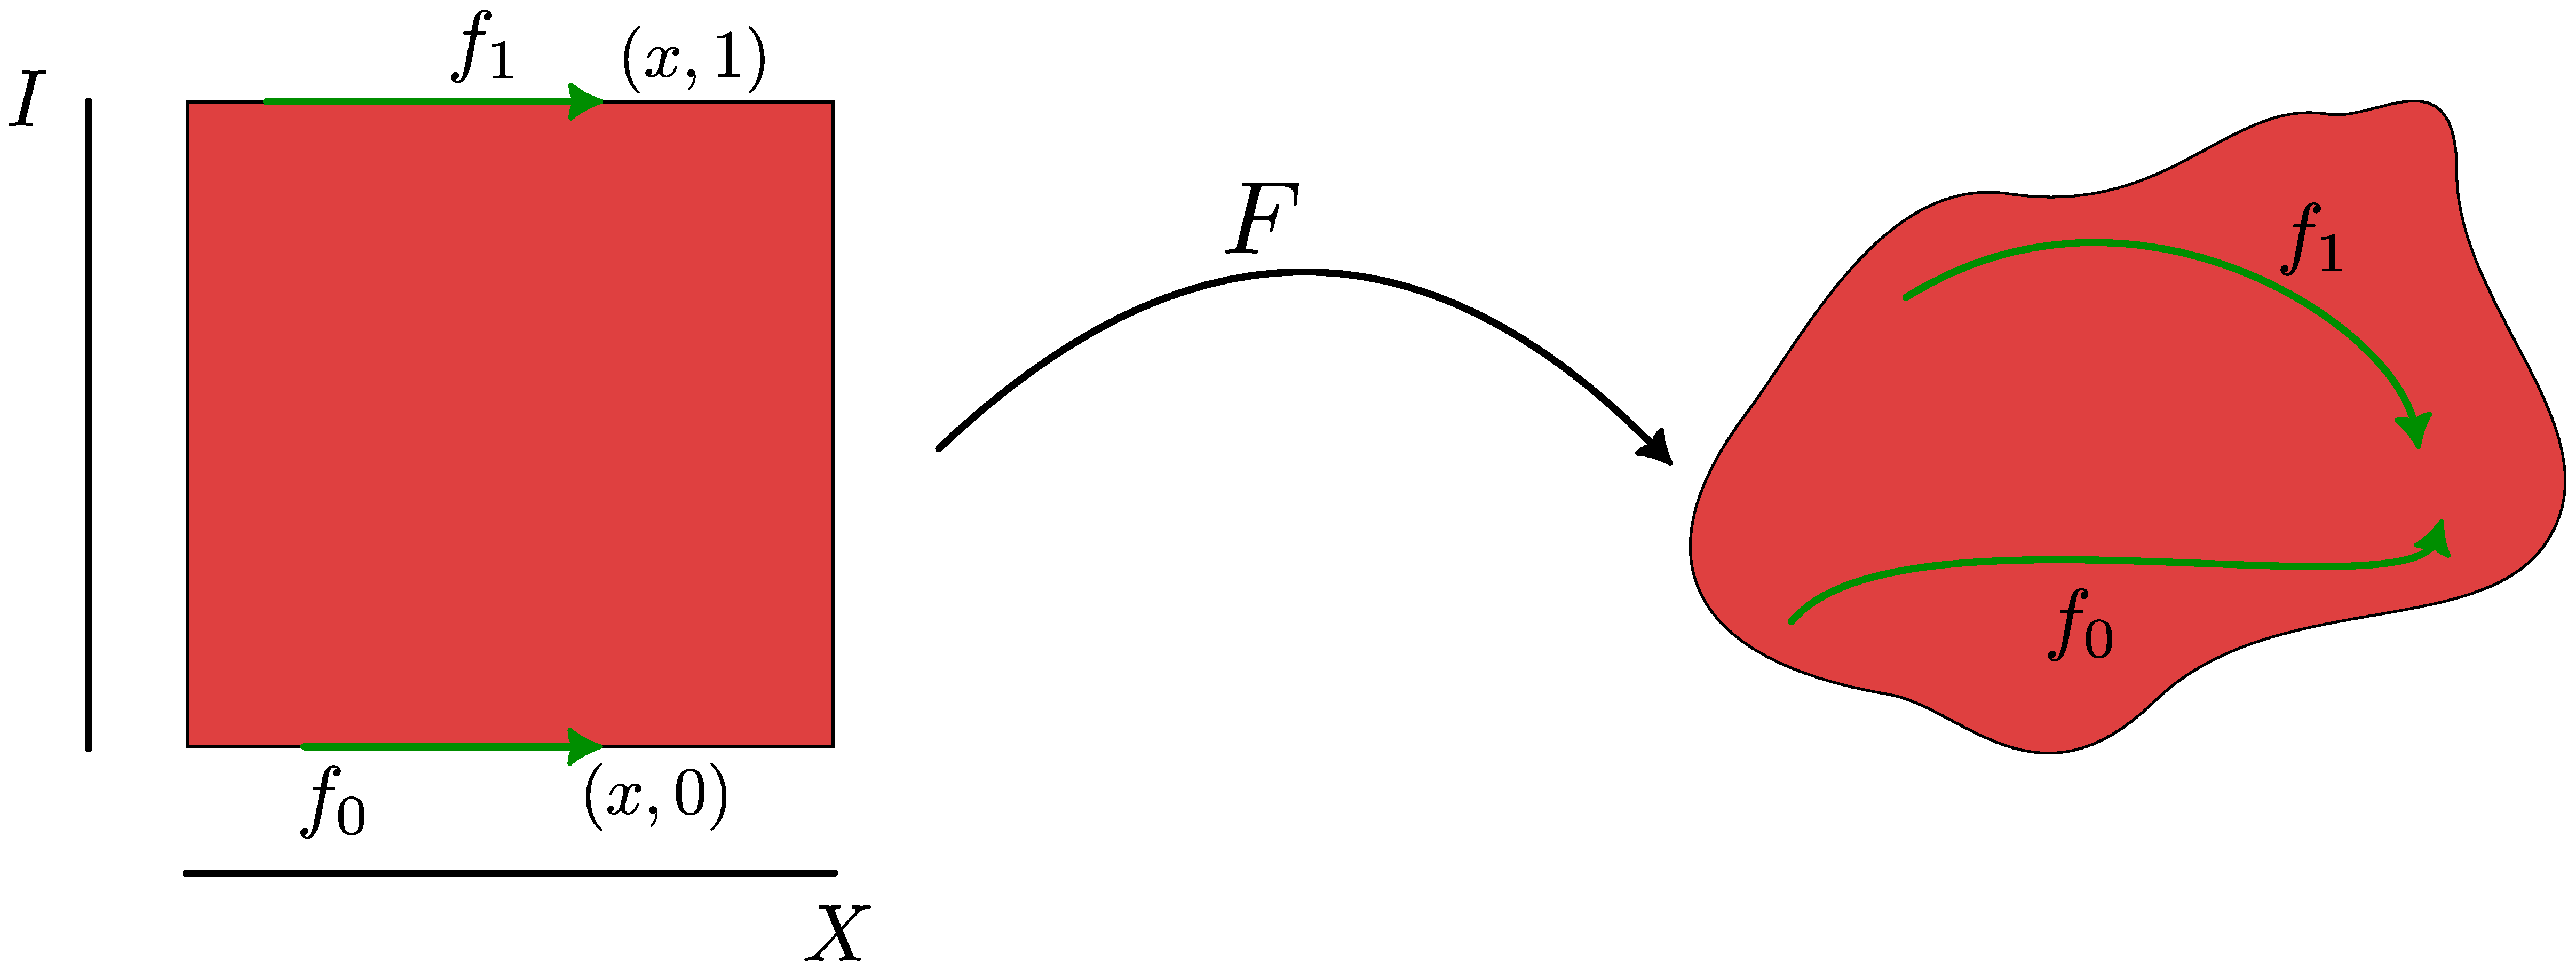
\includegraphics[scale=0.2]{Figures/homotopia.eps}
    \caption{Dos mapas continuas $f_0$ y $f_1$ homot\'opicos.}
    \label{fig_13}
\end{figure}

\begin{theorem}[Primer Teorema de Empaste]\label{thm_5.6}
    Sean $X$ y  $Y$ espacios topologicos y  $f:X \xrightarrow{} Y$ una mapa.
    Entonces:
    \begin{enumerate}
        \item[(1)] S\'i $\{U_\alpha\}$ es una colecci\'on de conjuntos abiertos
            de $X$ con  $X=\bigcup{U_\alpha}$, tal que $f|_{U_\alpha}$ es
            continua, entonces $f$ es continua.

        \item[(2)] S\'i $\{U_\alpha\}$ es una colecci\'on de conjuntos cerrados
            de $X$ con  $X=\bigcup{U_\alpha}$, tal que $f|_{U_\alpha}$ es
            continua, entonces $f$ es continua.
    \end{enumerate}
\end{theorem}

\begin{lemma}[Segundo Teorema de Empaste]\label{lemma_5.7}
    Sea $X$ un espacio topologico que es una union finita de conjuntos
    cerrados en $X$, $X=\bigcup_{i=1}^n{X_i}$. S\'i $Y$ es un espacio y
    $\{f_i\}_{i=1}^n$ una coleccion de mapas $f_i:X_i \xrightarrow{} Y$
    continuas que coincidan en la intersecci\'on, entonces existe una mapa
    continua $f:X \xrightarrow{} Y$ tal que $f|_{X_i}=f_i$.
\end{lemma}
\begin{proof}
    Considere la mapa $f(x)=f_i(x)$ para todo $x \in X_i$. Entonces $f$ coincida
    en la intersecci\'on con todo $f_i$, as\'i que es bien definida, y es claro
    que $f|_{X_i}=f_i$.

    Ahora sea $C$ un conjunto cerrado en  $Y$. Entonces  $\inv{f}(C)=X \cap
    \inv{f}(C)=\bigcup_{i=1}^n{X_i} \cap \inv{f}(C)=\bigcup_{i=1}^n{(X_i \cap
    f(C))}=\bigcup{(X_i \cap \inv{f_i}(C))}$. Ahora, $X_i$ y $\inv{f_i}$ est\'an
    cerrados as\'i que  $X_i \cap \inv{f_i}(X)$ es cerrado. Entonces el union
    finita de ellos para todo $i$ es cerrado, as\'i que $\inv{f}(C)$ es cerrado
    en $X$, lo cual hace  $f$ continua.
\end{proof}

\begin{lemma}[Tercer Teorema de Empaste]\label{lemma_5.8}
    Sea $X$ un espacio topologico que es una union arbitraria de conjuntos
    abiertos en $X$, $X=\bigcup{X_\alpha}$. S\'i $Y$ es un espacio y
    $\{f_\alpha\}$ una coleccion de mapas $f_\alpha:X_\alpha \xrightarrow{} Y$
    continuas que coincidan en la intersecci\'on, entonces existe una mapa
    continua $f:X \xrightarrow{} Y$ tal que $f|_{X_\alpha}=f_\alpha$.
\end{lemma}

\begin{lemma}\label{lemma_5.9}
    La homotop\'ia es una relaci\'on de equivalencia sobre mapas continuas.
\end{lemma}
\begin{proof}
    Sea $X$ y $Y$ espacios topologicos. Sea $f:X \xrightarrow{} Y$ una
    mapa continua y define $F:X \times I \xrightarrow{} Y$ con $F(x,t)=f(x)$
    para todo $(x,t) \in X \times I$. Nota que para alg\'un mapa continua $h:X
    \times I \xrightarrow{} X \times I$, que $F=\pi_1 \circ h$ donde $\pi_1$ es
    la proyecci\'on de la primer parte.$F$ es continua porque es la
    composici\'on de mapas continuas. Entonces vemos que $(x,t)
    \xrightarrow{h} (f(x),t) \xrightarrow{\pi_1} \xrightarrow{} f(x)$. Entonces
    podemos ver que $F(x,0)=F(x,1)=f(x)$, as\'i que $f \simeq f$.

    Ahora considere  $f:X \xrightarrow{} Y$, y $g:Y \xrightarrow{} Z$ continuas
    tal que $f \simeq g$. Sea  $F:X \times I \xrightarrow{} Y$ la homotop\'ia de
    esos dos mapas. Entonces $F(x,0)=f(x)$ y $F(x,1)=g(x)$. Defina la mapa $G:X
    \times I \xrightarrow{} Y$ dado por $G(x,t)=F(x,1-t)$. Como $G$ solo
    transforma coordinadas, $G$ es continua. Entonces vemos que
    $G(x,0)=F(x,1)=g(x)$ y $G(x,1)=F(x,0)=f(x)$; as\'i que $g \simeq f$.

    Por ultimo, sea  $f:X \xrightarrow{} Y$, $g:X \xrightarrow{} Y$ y $h:X
    \xrightarrow{} Y$ mapas continuas tales que $f \simeq g$ y $g \simeq h$.
    Entonces existe homotopias  $F:X \times I \xrightarrow{} Y$ y $G:X \times I
    \xrightarrow{} Y$ con $F(x,0)=f(x)$, $F(x,1)=g(x)$ y $G(x,0)=g(x)$,
    $G(x,1)=h(x)$. Considere la mapa $H:X \times I \xrightarrow{} Y$ dado por:
    \begin{equation*}
        H(x,t)=\begin{cases}
                F(x,2t), \text{ s\'i} 0 \leq t \leq \frac{1}{2} \\
                G(x,2t-1), \text{ s\'i } \frac{1}{2} \leq t \leq 1  \\
               \end{cases}
    \end{equation*}
    Vemos que los dominios de $F$ y $H$ coninciden, y que son continuas. As\'i
    que por la teorema del empaste, $H$ es continua. Entonces vemos que
    $H(x,0)=F(x,0)=f(x)$ y que $H(x,1)=G(x,1)=h(X)$ lo que hace $f \simeq h$.
\end{proof}

\begin{figure}[h]
    \centering
    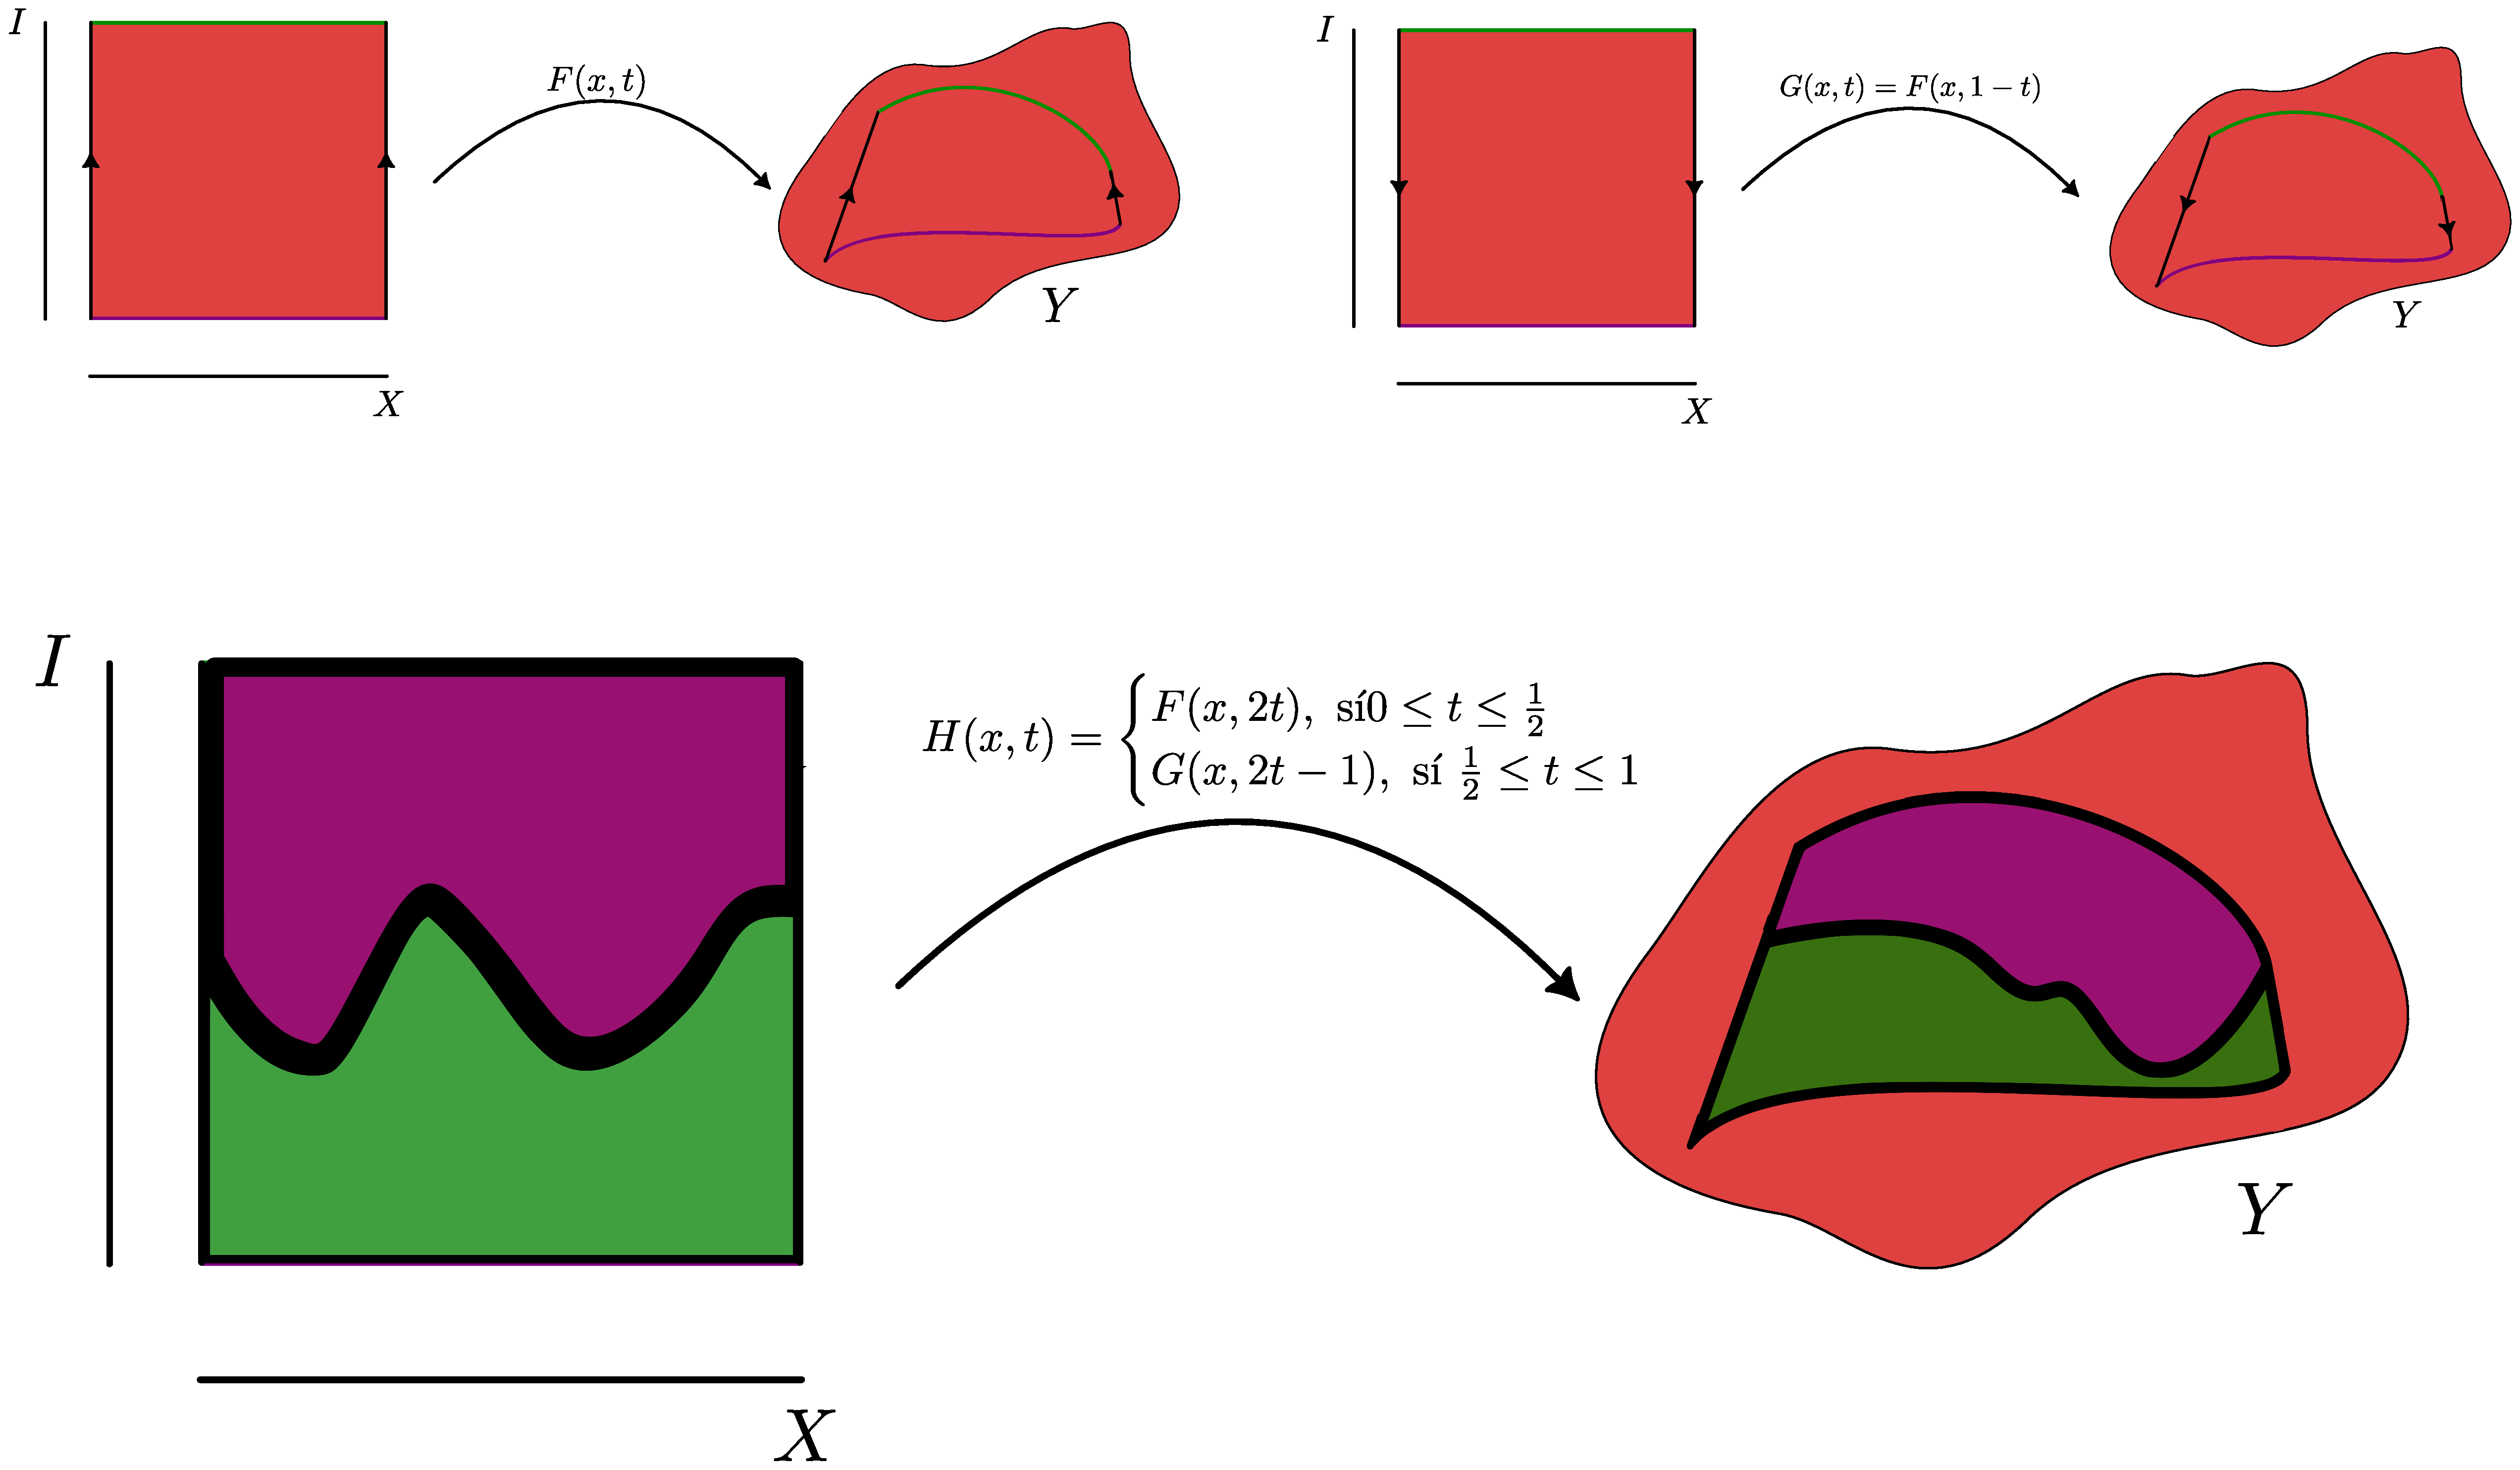
\includegraphics[scale=0.2]{Figures/homotopia_2.eps}
    \caption{La equivalencia de Homotop\'ia.}
    \label{fig_14}
\end{figure}

\begin{definition}
    Sea $X$ y  $Y$ espacios topologicos y  $f:X \xrightarrow{} Y$ una mapa
    continua. La \textbf{clase de homotop\'ia} de $f$ es el conjunto de todo
    mapa continua homotopico a $f$; es decir  $[f]=\{g:X \xrightarrow{} Y : g
    \text{ es continua y } g \simeq f\}$.
\end{definition}

\begin{theorem}\label{thm_5.10}
    Sean $X$ y  $Y$ espacios topologicos y sea  $f_i:X \xrightarrow{} Y$ y
    $g_i:X \xrightarrow{} Y$ mapas continuas para todo $i \in \faktor{\Z}{2\Z}$.
    S\'i $f_0 \simeq f_1$ y $g_0 \simeq g_1$, entonces tenemos que $g_0 \circe
    f_0 \simeq g_1 \circ f_1$.
\end{theorem}
\begin{proof}
    Sean $F:X \times I \xrightarrow{} Y$  y $G:X \times I \xrightarrow{} Y$
    homotopias entre $f_0,f_1$ y $g_0,g_1$, respectivamente. Afirmamos que $g_0
    \circ f_0 \simeq g_1 \circ f_0$. Sea $H:X \times I \xrightarrow{} Y$ la mapa
    definida como $H=G \circ f_0$. Es decir que $H(x,t)=G(f_0(x),t)$. Nota que
    como $G$ y  $f_0$ son continuas, entonces $H$ es continua, y que
    $H(x,0)=G(f_0(x),0)=g_0 \circ f_0(x)$ y $H(x,1)=G(f_0(x),1)=g_1 \circ
    f_0(x)$. As\'i que $g_0 \circ f_0 \simeq g_1 \circ f_0$.

    Ahora afirmamos que $g_1 \circ f_0 \simeq g_1 \circ f_1$. Considere $K:X
    \times I \xrightarrow{} Y$ dado por $K=g_1 \circ F$. Como $g_1$ y $F$ son
    continuas, tenemos $K$ continua. Entonces  $K(x,0)=g_1 \circ f_0(x)$ y
    $K(x,1)=g_1 \circ f_1(x)$. Entonces $g_1 \circ f_0 \simeq g_1 \circ f_1$.
    Por lo tanto, como homotopia es transitiva, obtenemos que $g_0 \circ f_0
    \simieq g_1 \circ f_1$.
\end{proof}
\begin{corollary}
    Homoto\'ia defina una congruencia en la categor\'ia $\Top$.
\end{corollary}

\begin{definition}
    Definimos el \textbf{categor\'ia homot\'opico} de ser la categor\'ia
    cociente de $\Top$ bajo homotop\'ia, y lo denotamos  $\text{hTop}$.
\end{definition}

\begin{definition}
    Una mapa continua $f:X \xrightarrow{} Y$ es una \textbf{equivalencia de
    homotop\'ia} s\'i existe un $g:Y \xrightarrow{} X$ tal que $g \circ f \simeq
    1_X$ y  $f \circ g \simeq 1_Y$. Decimos entonces que $X$ es de la misma
    \textbf{tipo de homotop\'ia} que $Y$.
\end{definition}

\begin{example}\label{}
    Un circulo y un disco perforado no son homeomorfos, per s\'i son del mismo
    tipo de homotopia.
    \begin{figure}[h]
        \centering
        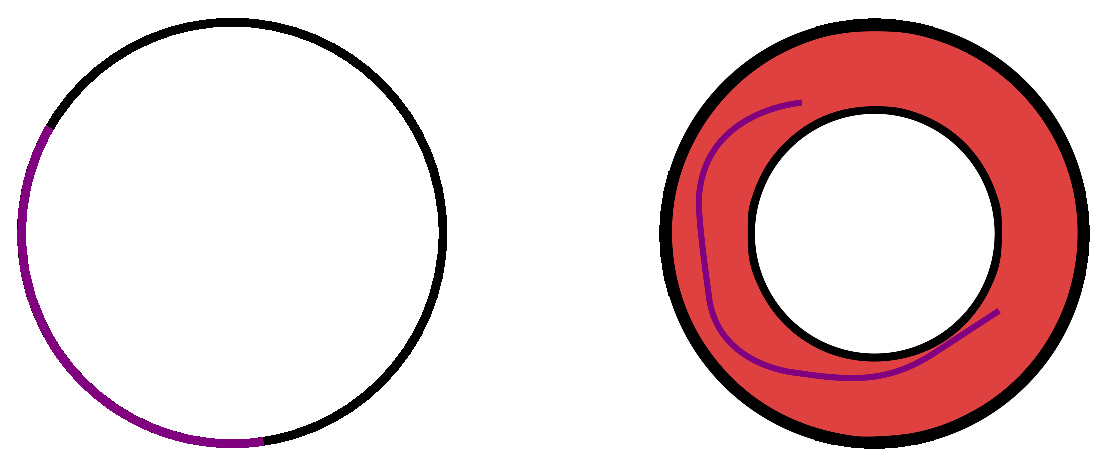
\includegraphics[scale=0.5]{Figures/homotopy_equivalence.eps}
        \caption{}
        \label{fig_15}
    \end{figure}
\end{example}

\begin{definition}
    Sean $X$ y  $Y$ espacios topologicos. Decimos que un mapa $f:X
    \xrightarrow{} Y$ es \textbf{homotopicamente nula} s\'i es homotopico a una
    mapa constante en $Y$.
\end{definition}

\begin{theorem}[La Teorema Fundamental del Algebra]\label{thm_5.11}
    Todo polinomio con coeficientes complejas tiene al menos una ra\'iz
    complejo.
\end{theorem}

\section*{Lectura 6: Sumas Directas y Productos Semidirectas.}

\section*{Lectura 7: Acciones de Grupos.}

\begin{theorem}[EL Teorema de Cayley]\label{thm_7.26}
    Todo grupo es isomorfo a un subgrupo del grupo de simetrico.
\end{theorem}
\begin{proof}
    Sea $G$ un grupo y  $A(G)$ el grupo simetrico de $G$. Defnia $\lambda:G
    \xrightarrow{} A(G)$ dado por $g \xrightarrow{} \lambda_g$, donde
    $\lambda_g:G \xrightarrow{} G$ esta dado por $x \xrightarrow{} gx$. Note que
    $\lambda_g$ es un permutacion de los elementos de  $G$, es sobre, y es 1--1
    por cancelacion, as\'i que  $\lambda_g \in A(G)$. As\'i que $\lambda$ es
    bien definido.

    Ahora suponga que que  $\lambda(g)=\lambda(h)$, entonces para alg\'un $x \in
    G$,  $\lambda_g(x)=\lambda_g(h)$, pues $gx-gh$. Por cancelaci\'on, tenemos
    que  $g=h$. s\'i que  $\lambda$ es 1--1. Ahora dado  $x \in G$, que
    $\lamda(gh)(x)=\lambda_{gh}(x)=(gh)x=g(hx)=g(\lamda_h(x))=\lambda_g(\lambda_h(x))=
    \lambda_G\lambda_h(x)$. As\'i que $\lambda$ definia  una isomorfismo de $G$
    hac\'ia  $\lambda(G)$ lo cual es subgrupo de $A(G)$.
\end{proof}

\begin{example}\label{}
    Por la teorema de Cayley, tenemos que $D_3 \simeq S_6$.
\end{example}

\begin{definition}
    Un grupo $G$  \textbf{actua} sobre un conjunto $X$ s\'i para todo  $g \in
    G$, existe una mapa  $G \times X \xrightarrow{} X$ dado por $(g,x)
    \xrightarrow{} g \cdot x$ tal que:
    \begin{enumerate}
        \item[(1)] $h \cdot (g \cdot x)=(hg) \cdot x$.

        \item[(2)] $e \cdot x=x$ para todo  $x \in X$.
    \end{enumerate}
\end{definition}

\begin{example}\label{}
    \begin{enumerate}
        \item[(1)] Todo grupo actua sobre si mismo bajo multiplicacion pr la
            izquierda. Llamamos esto el \textbf{accion regular}.

        \item[(2)] Todo grupo actua sobre si mismo via la accion de
            \textbf{conjugacion} definido pro $(g,x) \xrightarrow{} gx\inv{g}$.
            Nota que $h \cdot (g \cdot x)=h \cdot
            (gx\inv{g})=hgx\inv{g}\inv{h}=(hg)x\inv{(hg)}=(hg) \cdot x$. Tambein
            $e \cdot x=ex\inv{e}=x$.
    \end{enumerate}
\end{example}

\begin{definition}
    Definimos el \textbf{kernel} de una accion $G \times X \xrightarrow{} X$ de
    ser el conjunto $\ke=\{g \in G: g \cdot x=x\}$.
\end{definition}

\begin{example}\label{}
    S\'i $G$ actua sobre si mismo via conjugacion, entonces si  $gx\inv{g}=x$,
    tenemos que $gx=xg$ para todo  $x \in G$. Por lo tanto  $\ker=\{g \in G :
    gx=xg \text{ para todo } x \in G\}$. Llamamos este kernel el \textbf{centro}
    de $G$, y lo denotamos como  $Z(G)$.
\end{example}

\section*{Lectura 8: Las Teoremas de Sylow}

\begin{definition}
    Sea $p \in \Z^+$ un primo. Llamos a un grupo $G$ un \textbf{$p$-grupo} s\'i
    cada $g \in G$ es una potencia de  $p$.
\end{definition}

\begin{example}\label{}
    \begin{enumerate}
        \item[(1)] El grupo Klein $V_4=\faktor{\Z}{2\Z} \oplus \faktor{\Z}{2\Z}$
            es un $2$-grupo.

        \item[(2)] Los grupose $\faktor{\Z}{14\Z} \oplus \faktor{\Z}{2\Z}$ y
            $D_{16}$ son $2$-grupos.

        \item[(3)] El grupo $\bigoplus_{n=1}^{\infty}{\faktor{\Z}{5^n\Z}}$ es un
            $5$-grupo, pero  $\prod_{n=1}^{\infty}{\faktor{\Z}{5^n\Z}}$ solo es
            un $5$-grupo cuando $n=1$.
    \end{enumerate}
\end{example}

\begin{definition}
    S\'i $G$ es un grupo con orden  $p^rm$ donde  $p$ es primo y  $p \not| m$,
    entonces llamamos un subgrupo  $P \leq G$ un \textbf{$p$-subgrupo de Sylow},
    o un \textbf{$p$-Sylow} s\'i $\ord{P}=p^r$.
\end{definition}

\begin{lemma}\label{8.31}
    S\'i $G$ es u grupo de orden  $p^rm$ con  $p$ primo, y $p \not|m$ y $P \leq
    G$ es un  $p$-Sylow de  $G$, entonces  $P$ es de orden lo maximo posible.
\end{lemma}
\begin{proof}
    Por el teorema de Lagrange.
\end{proof}

\begin{example}\label{}
    $|D_6|=2^2 \cdot 3$. Nota que $P_1=\{e,r^3,tr^3t\}$,
    $P_2=\{e,r^3,rt,r^4t\}$, y $P_3=\{e,r^3,r^2t,r^5t\}$ son $2$-Sylows de
    $D_6$ y $P=\{e,r,r^4\}$ es $3$-Sylow.
\end{example}

\begin{lemma}\label{8.32}
    S\'i $n=p^rm$ con  $p$ primo y  $p \not| m$, entonces
    \begin{equation*}
        {n \choose p^r} \equiv m \mod{p}
    \end{equation*}
\end{lemma}
\begin{proof}
    Nota que $(x+1)^{p^r}=\sum_{k=1}^{p^r}{{p^r \choose k}x^{p^r-k}}
    \equiv x^{p^rm}+1 \mod{p}$. Entonces $(x+1)^{p^rm} \equiv (x^{p^r}+1)^m
    \mod{p}$, as\'i que
    \begin{equation*}
        \sum{{p^rm \choose k}x^{p^rm-k}} \equiv \sum{{m \choose
        k}(x^{p^r})^{m-k}} \mod{p}
    \end{equation*}
    Mirando el coeficiente de $x^{p^r}$, en la izquierd, tenemos que este
    termino occure cuando $k=p^r(m-1)$, y obtenemeos ${p^rm \choose p^r}={n
    \choose p^r}$. Por el lado derecho, el termino $x^{p^r}$ occure cuando
    $k=m-1$ y por simetria obtenemos ${m \choose 1}=m$.
\end{proof}

\begin{theorem}[El Primer Teorema de Sylow]\label{8.33}
    Sea $G$ un grupo finito de orden  $p^rm$ donde  $p$ es primo, y  $p \not|
    m$. Entonces existe al menos un  $p$-subgrupo de Sylow, de  $G$.
\end{theorem}
\begin{proof}
    Sea $X={G \choose p^r}$. Note que $G$ actua sobre  $X$ v\'a la
    multiplicacion por la izquierda. Ahora, este accion induce en  $X$ una
    particion de  $X$ en orbitas. Es decir
    \begin{equation*}
        {G \choose p^r}=\bigcup{\Oc(S)}
    \end{equation*}
    entonces $p \not| \sum{|\Oc(S)|}$. Por lo tanto, existe un $S \in X$ con $p
    \not| |\Oc(S)|$. Sea $P=\stab{S}$ Entonces por el teoream del
    \'orbita-estabilizador, tenemos
    \begin{equation*}
        |\Oc(S)|=\frac{\ord{G}}{\ord{P}}=\frac{p^rm}{\ord{P}}
    \end{equation*}
    Como $p \not| |\Oc(S)|$, $\ord{P}$ tiene que ser un multiplo de $p^r$, es
    decir que $p^r | \ord{P}$, por lo tanto $p^r \leq \ord{P}$.

    Por otro lado, defina la mapa $\lambda_x:P \xrightarrow{} S$, para $x \in S$
    dado por $\lambda_x:g \xrightarrow{} \lambda_x(g)=g \cdot x$. Vemos que esta
    mapa es bien definida, y que es 1--1. Por lo tanto $\ord{P} \leq |S|=p^r$.
    Por lo tanto $P$ es un  $p$-subugrupo de Sylow.
\end{proof}

\section*{Lectura 9: Grupos Simples}

\begin{definition}
    Un grupo $G \neq \langle e \rangle$ es \textbf{simple} s\'i sus unicons
    subgrupos normales son el mismo y $\langle e \rangle$.
\end{definition}

\begin{example}\label{}
    \begin{enumerate}
        \item[(1)] $\faktor{\Z}{5\Z}$ tiene como subgrupos $\langle 0 \rangle$ y
            $\faktor{\Z}{5\Z}$. Entonces $\faktor{\Z}{5\Z}$ es simple.

        \item[(2)] El grupo dihedral $D_n$ no es normal porque tiene  $\langle r
            \rangle$ como subgrupo simple; pues $[D_n:\langle r \rangle]=2$.
    \end{enumerate}
\end{example}

\begin{lemma}\label{9.38}
    S\'i $P$ es un  $p$-grupo finito no trivial, entonces $Z(P)$ no es trivial.
\end{lemma}
\begin{proof}
    Deje que $P$ actue sobre si mismo via conjugacion. Las \'orbitas de este
    accion son las clases de conjugacion $\cl{g}$, donde $g \in P$. Tenemos que
    $x \in P$ esta en una clase de tama\~no  $1$ s\'i y solo s\'i $x \in Z(P)$.
    Por el teorema del \'orbita-estabilizador, tenemos que el tama\~no de los
    $\cl{g}$ divide a $\ord{P}=p^r$, donde $p,r \in \Z^+$ y $p$ es primo.

    Ahora, s\'i  $Z(P)=\langle e \rangle$, entonces hay una sola \'orbita de
    tama\~no $1$. Entonces los demas $\ord{\cl{x}} | \ord{P}$. Esto es una
    contradicci\'on de que $P$ es un $p$-grupo.
\end{proof}
\begin{corollary}
    S\'i $P$ es un $p$-grupo  no isomorfo a $\faktor{\Z}{p\Z}$, para $p$ primo,
    entonces  $P$ no es simple.
\end{corollary}
\begin{proof}
    Nota que $Z(P) \unlhd P$.
\end{proof}

\begin{lemma}\label{9.39}
    El subgrupo $P$ de un grupo $G$ es un $p$-Sylow normal de $G$ s\'i y solo
    s\'i es el \'unico $p$-Sylow de $G$.
\end{lemma}

\begin{lemma}\label{9.40}
    Sea $G$ un grupo finito noabeliano y simple. S\'i  $p|\ord{G}$, para $p$
    primo, entonces  $n_p(G)>1$.
\end{lemma}
\begin{proof}
    S\'i $p$ es unico, entonces $\ord{G}=p^r$ y $G$ es un  $p$-grupo no trivial.
    Entonces  $Z(G)$ tambien no es trivial. Como $Z(G) \unlhd G$ y $G$ es
    simple entonces $Z(G)=G$, lo cual no puede pasar.

    Ahora, s\'i $P$ es un  $p$-Sylow de $G$, entonces  $\langle e \rangle \leq P
    \leq G$, donde la segundo inclusi\'on es estricta. S\'i $n_p(G)=1$, entonces
     $P \unlhd G$, lo cual no puede pasar. Por lo tanto  $n_p(G)>1$.
\end{proof}

\begin{lemma}\label{9.31}
    Sea $G$ un grupo de orden $pq$, donde $p$ y  $q$ son primos distintos.
    Entonces:
    \begin{enumerate}
        \item[(1)] S\'i $q \not\equiv 1 \mod{p}$, entonces $G$ tiene un
            $p$-Sylow normal.

        \item[(2)] S\'i $q \not\equiv 1 \mod{p}$, y $p \not\equiv 1 \mod{q}$,
            entonces $G$ es ciclico.

        \item[(3)] $G$ no es simple.
    \end{enumerate}
\end{lemma}
\begin{proof}
    Note que $n_p(G) \equiv 1 \mod{p}$ y $n_p(G)|q$ por el tercer teorema de
    Sylow. Entonces o $n_p(G)=1$, o $n_p(G)=q$. Como $q \not\equiv 1 \mod{p}$,
    tenemos que $n_p(G)=1$ y $G$ tiene un unico  $p$-Sylow, y es normal.

    Ahora, suponga que $q \not\equiv 1 \mod{p}$ y $p \not\equiv 1 \mod{q}$.
    Tenemos que $G$ tiene un  $p$-Sylow unico $P$, y un  $q$-Sylow unico $Q$.
    Mas a\'un $P$ y  $Q$ son ciclicos. Existen  $x \in P$ y  $y \in Q$ con
    $P=\langle x \rangle$ y $Q=\langle y \rangle$. Por supuesto $\ord{P}=p$ y
    $\ord{Q}=q$. Ahora, como $P,Q \unlhd G$ y $P \cap Q=\langle e \rangle$
    entonces tenemos que $xy=yx$; entonces  $(xy)^n=x^ny^n$. Por lo tanto
    $(xy)^{pq}=e$. Esto hace $G$ ciclico.

    Por ultimo, sin perder la generalidad, asume que  $p>q$. Por lo tanto,
    tenemos que  $p \not|q-1$ y  $q \not\equiv 1 \mod{p}$. Por arriba, $G$ tiene
    un unico  $p$-Sylow normal, lo que hace que $G$ no sea simple.
\end{proof}

\begin{lemma}\label{9.42}
    Sea $G$ un grupo con noabeliano orden $p^2q$ con  $p$ y  $q$ primos
    distintos. Entonces $G$ contiene un  $p$-Sylow normal o un $q$-Sylow normal.
\end{lemma}
\begin{proof}
    Supong lo contrario. Sea $n_p(G)>1$ y $n_q(G)>1$. Note que un $q$-Sylow
    tiene orden $q$, y por lo tanto es ciclico. Entonces tenemos  $q-1$
    elementos de orden $q$. Entonce cualquier $y$ del  $q$-Sylow genera un unico
     $q$-Sylow. Por lo tanto  $q=n_q(q-1)$. Ahora, $n_q(G)|p^2$ as\'i que o
     $n_q(G)=p$ o  $n_q(G)=p^2$. S\'i $n_q(G)=p^2$, entonces el unmero de
     elementos de orden diferente a $q$ es  $p^2q-p^2(q-1)=p^2$ lo que dice que
     hay un $p$-Sylow unico. Por lo tanto, $G$ no es simple.

     Por otro lado, s\'i  $n_q(G)=p$, entonces $n_q(G) \equiv 1 \mod{q}$ y $p
     \equiv 1 \mod{q}$, lo que dice $p>q$. Peron  $n_p(G)|q$ y como $q$ es
     primo, entonces $n_p(G)=q$, luego, $n_p(G) \equiv 1 \mod{p}$ implica que $q
     \equiv 1 \mod{p}$ lo que dice que $q>p$.  Una contradiccion.
\end{proof}
\begin{corollary}
    $G$ no es simple.
\end{corollary}

\begin{example}\label{}
    \begin{enumerate}
        \item[(1)] Por los resultados arriba, el primer grupo noabeliano simple
            es el grupo $A_5$ de orden $60=2^2 \cdot 3 \cdot 5$.

        \item[(2)] Suponga que $G$ es u grupo de orden  $2552=2^3 \cdot 11 \cdot
            29$. Suponiendo que  $G$ es simple, entonces  $n_{11}>1$ y
            $n_{29}>1$. Ahora, como $n_{11}(G) \equiv 1 \mod{11}$, y
            $n_{11}(G)|2^3 \cdot 29$. los divisores positivos de $8 \cdot 29$
            son dados por
            \begin{align*}
                1   &&  2   &&  4   &&  8   &&  29  &&  58  &&  116 &&  232 \\
            \end{align*}
            Por lo tanto $n_{11}(G)=232$, y hay $232$  $11$-Sylows. Como el
            orden de cada uno de ellos es  $11$, entonces ellos son ciclicos,
            con interseccion trivial entre ellos, y por lo tanto $G$ tiene
            $2320$ elementos de orden  $11$.

            Por el mismo lado, tenemos  $n_{29} \equiv 1 \mod{29}$ y  $n_{29}|8
            \cdot 11$ lo que tiene divisores
            \begin{align*}
                1   &&  2   &&  4   &&  8   &&  11  &&  22  &&  44  &&  88  \\
            \end{align*}
            As\'i que $n_{29}=88$ y $G$ tiene  $2464$ elementos de orden  $29$.
            Por lo tanto  $\ord{G} \geq 2320+2464>2552$ una contradiccion. As\'i
            que $G$ no es simple.
    \end{enumerate}
\end{example}

\section*{Lectura 10: El Teorema de Jordan-H\"older}

\begin{definition}
    Sea $G$ un grupo y  $G_0, \dots, G_n$ donde $G_n=\langle e \rangle$ y
    $G_0=G$ tal que $G_{i+1} \unlhd G_i$. Entonces se llama el serie
    \begin{equation*}
        G_n \unlhd \dots \unlhd G_0
    \end{equation*}
    una \textbf{serie subnormal} de $G$.
\end{definition}

\begin{example}\label{}
    \item[(1)] Coje $G_0=D_8$, $D_1=\langle r \rangle$, $G_2=\langle r^2
        \rangle$, $G_3=\langle r^4 \rangle$ y $G_4=\langle e \rangle$. Entonces
        $G_4 \unlhd G_3 \unlhd G_2 \unlhd G_1 \unlhd G_0$.
\end{example}

\end{document}
